Um escoamento em uma cavidade onde as parades laterais e inferior
permanecem imóveis e a tampa se desloca com velocidade constante
tal como \textit{$U_{top} = 1$} é conhecido como \textit{Escoamento em uma Cavidade de Tampa Móvel} 
(\textit{lid-driven cavity flow}). 
A \ref{cavity} apresenta esquematicamente este escoamento e
o perfil do campo de velocidade esperado.

\vspace{1cm}
\begin{figure}[H]
\begin{center}
\begin{tikzpicture}[scale=1.1]
 \draw [pattern=north east lines] (0,-0.1) -- (3,-0.1) -- (3,3) -- (2.9,3) -- (2.9,0) -- (0.1,0) -- (0.1,3) -- (0,3) -- cycle;
 \draw [pattern=north east lines] (-0.1,3) -- (-0.1,3.1) -- (3.1,3.1) -- (3.1,3) -- cycle;

 \draw [->,thick] (3.2,3.05)--(4.2,3.05) node[above] {$U_{top}$};

 \draw [->,thick] (2.4,2.4) arc (45:-180:1.2);
 
 \draw [->,thick] (-2,-0.1)--(-2,1.5) node[left] {$y$};
 \draw [->,thick] (-2.1,0)--(-0.5,0) node[below] {$x$};

\end{tikzpicture}
\end{center}
\caption{Escoamento em uma Cavidade com tampa móvel}
\label{cavity}
\end{figure}

\vspace{0.5cm}
Foram simulados os escoamentos com
os seguintes número de Reynolds (\textit{Re}): 10, 100, 400 e 1000. Os
resultados obtidos foram comparados com Ghia et al. (1982) \cite{ghia1982} e Marchi et al. (2009) \cite{marchi2009}.
O domínio foi discretizado utilizando uma malha 
triangular linear com 1563 nós e 2988 elementos. 

\medskip
\noindent
As condições de contorno utilizadas foram:

\begin{itemize}
     \item \textit{condição de não escorregamento}: esta condição é utilizada nas placas laterais e inferior, 
      onde todas as componentes da velocidade são especificadas
      com os valores $u=0$ e $v=0$.
      A função de corrente também é espeficado com o valor de $\psi=0$.

     \item \textit{condição de movimentação da parede}: esta condição é utilizada na placa superior, 
      onde todas as componentes da velocidade são especificadas
      com os valores $u=1$ e $v=0$.
      A função de corrente também é espeficado com o valor de $\psi=0$.
\end{itemize}


\newpage
As \ref{velocity vx cavity} e \ref{velocity vy cavity} apresentam 
o perfil de $u$ e de $v$, respectivamente, em regime permanente para vários números de Reynolds.
Os resultados obtidos são comparados com os resultados de Ghia et al. (1982) \cite{ghia1982} e Marchi et al. (2009)  \cite{marchi2009}.
Na \ref{countours streamfunction}, é apresentado os contornos da função de corrente para os Reynolds analisados.

\begin{center}
\begin{figure}[H]
     \centering
     \begin{minipage}{.5\linewidth}
      \centering
      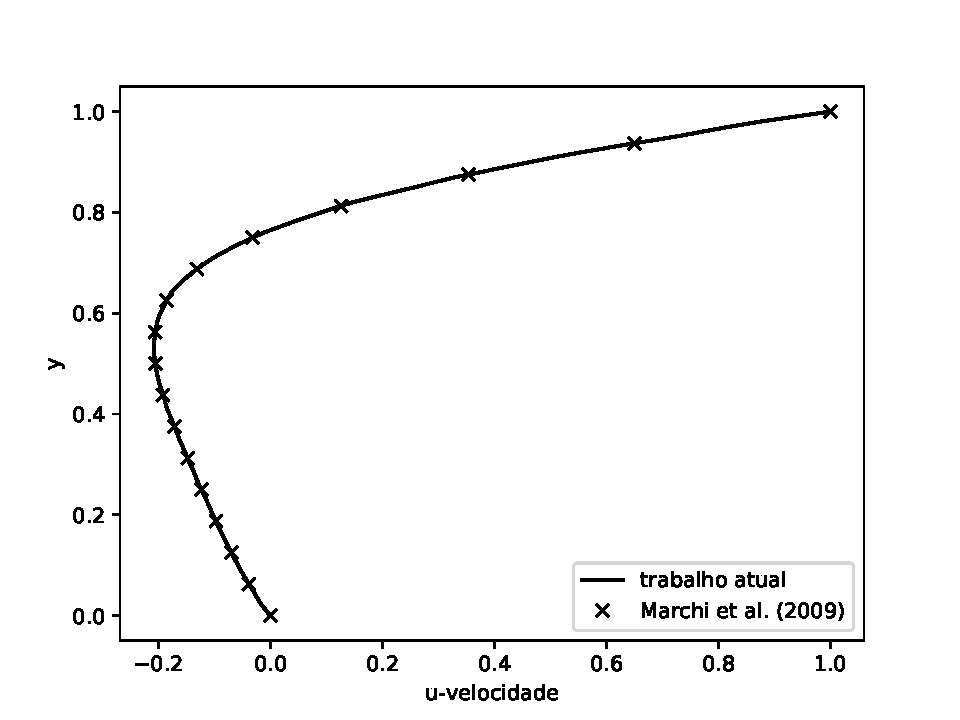
\includegraphics[scale=0.53]{./02_chaps/cap_validation/figure/Re_10_u_profile.pdf}\\
      (a)
     \end{minipage}%
     \begin{minipage}{.5\linewidth}
      \centering
      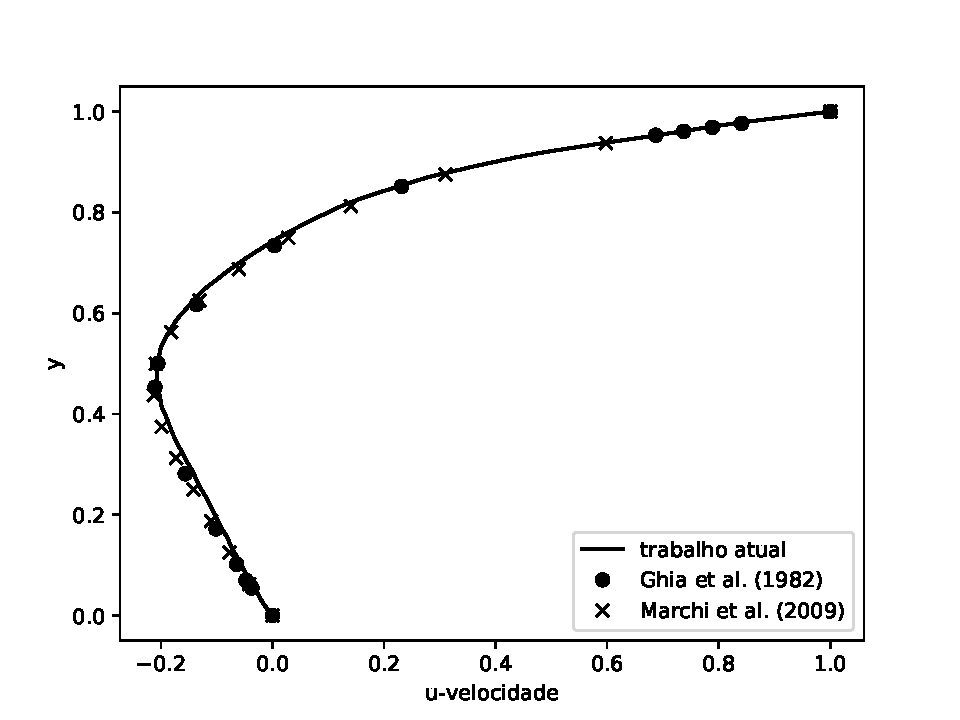
\includegraphics[scale=0.53]{./02_chaps/cap_validation/figure/Re_100_u_profile.pdf}\\
      (b)
     \end{minipage}
     \begin{minipage}{.5\linewidth}
      \centering
      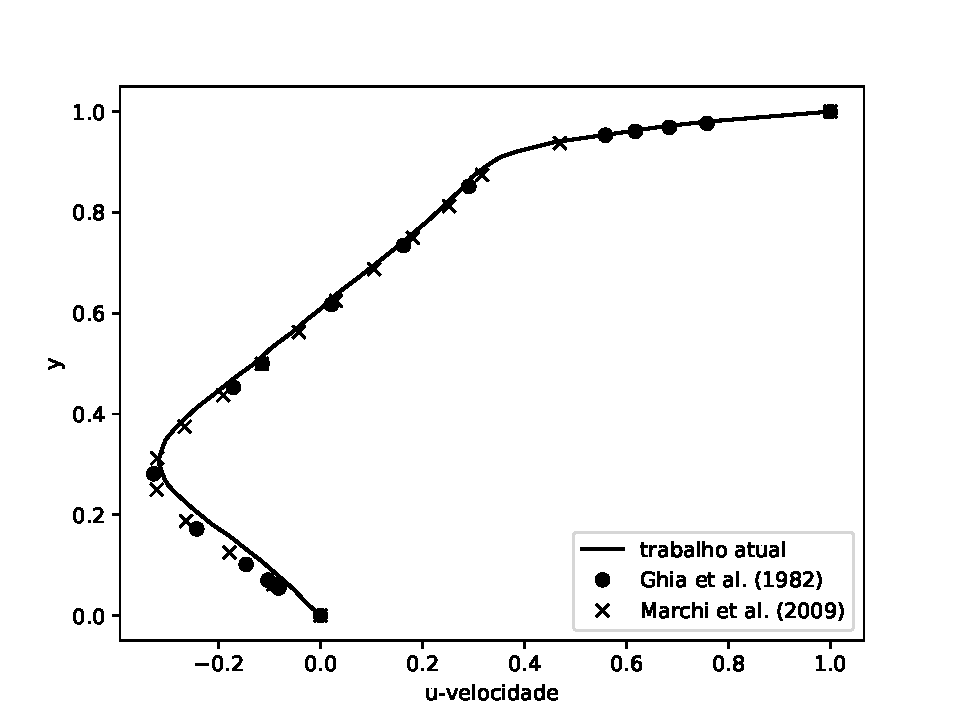
\includegraphics[scale=0.53]{./02_chaps/cap_validation/figure/Re_400_u_profile.pdf}\\
      (c)
     \end{minipage}%
     \begin{minipage}{.5\linewidth}
      \centering
      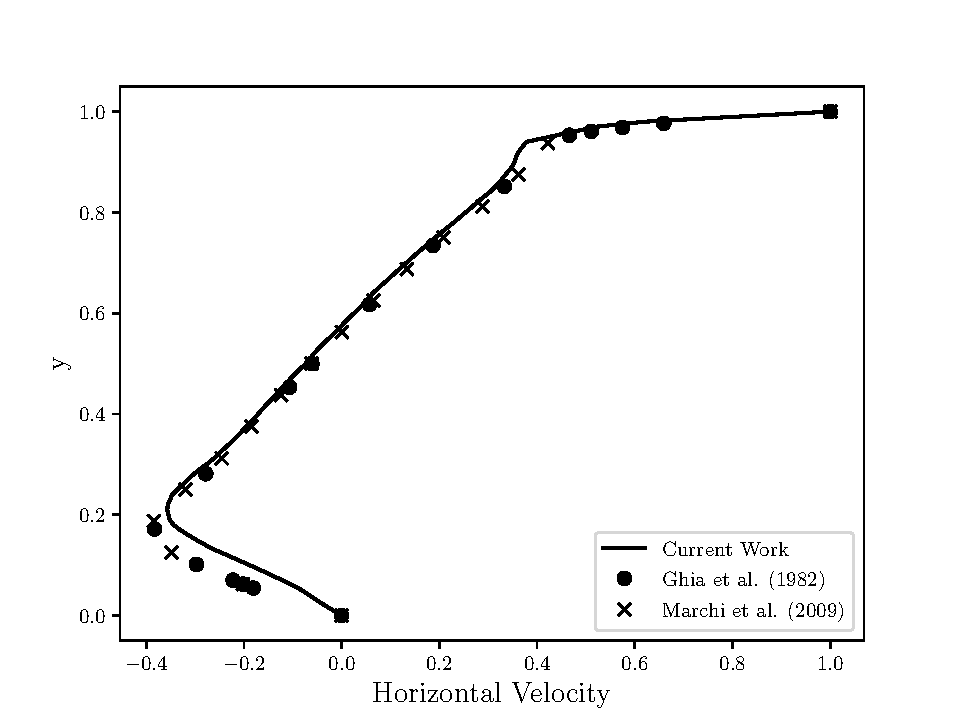
\includegraphics[scale=0.53]{./02_chaps/cap_validation/figure/Re_1000_u_profile.pdf}\\
      (d)
     \end{minipage}
     \medskip
     \caption{Perfil de $u$ na linha central da cavidade ($x=0.5$) com diferentes Reynolds:
     (a) 10
     (b) 100
     (c) 400
     (d) 1000.}
     \label{velocity vx cavity}
\end{figure}
\end{center}

\begin{figure}[H]
     \centering
     \begin{minipage}{.5\linewidth}
      \centering
      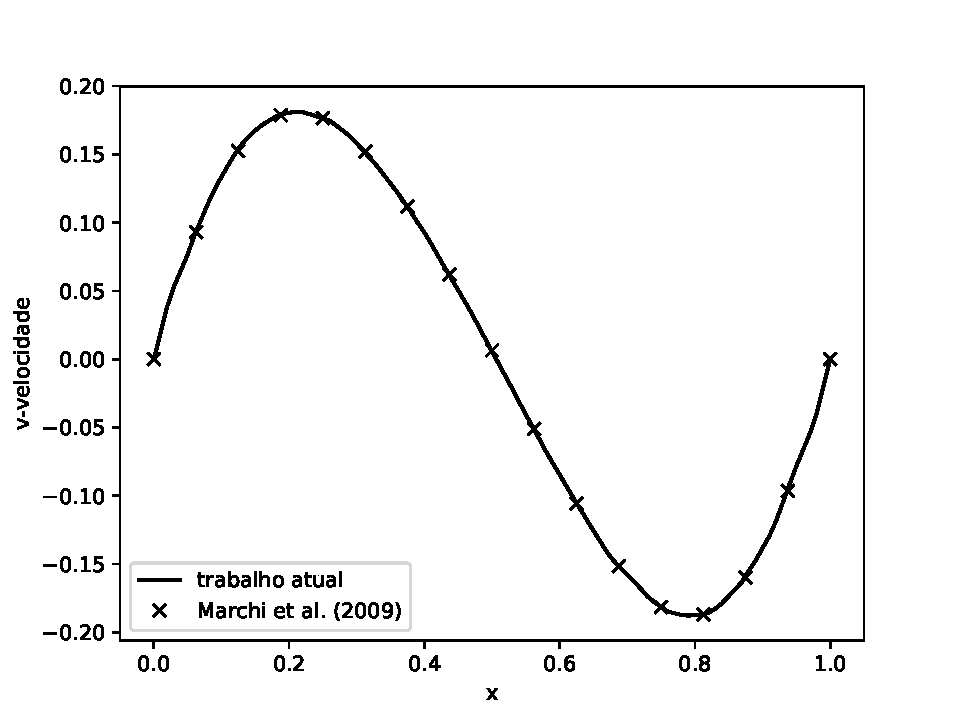
\includegraphics[scale=0.53]{./02_chaps/cap_validation/figure/Re_10_v_profile.pdf}\\
      (a)
     \end{minipage}%
     \begin{minipage}{.5\linewidth}
      \centering
      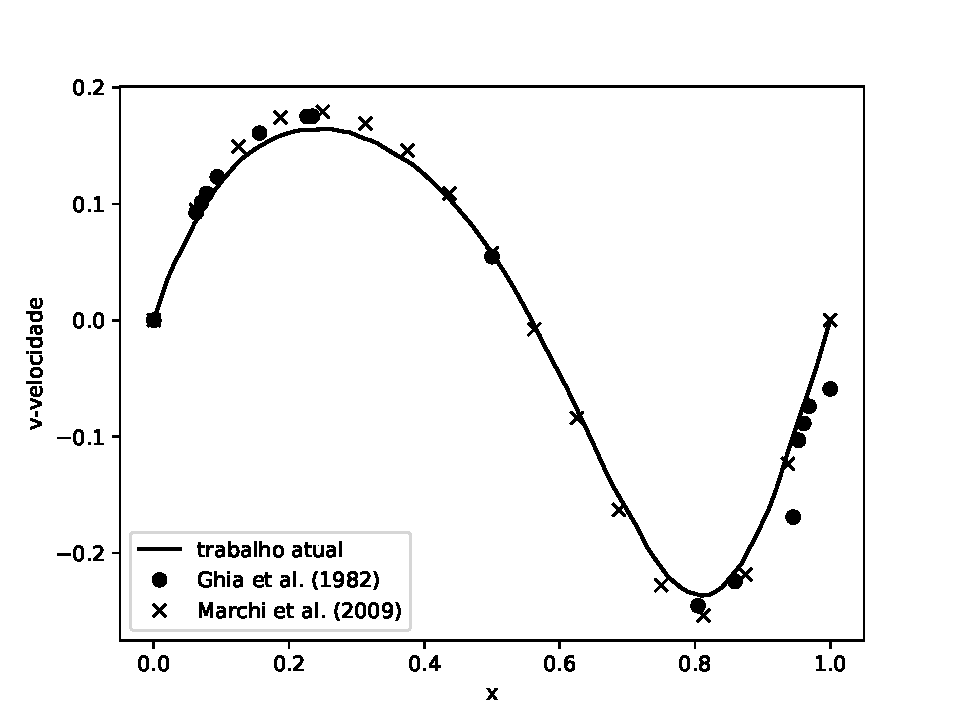
\includegraphics[scale=0.53]{./02_chaps/cap_validation/figure/Re_100_v_profile.pdf}\\
      (b)
     \end{minipage}
     \begin{minipage}{.5\linewidth}
      \centering
      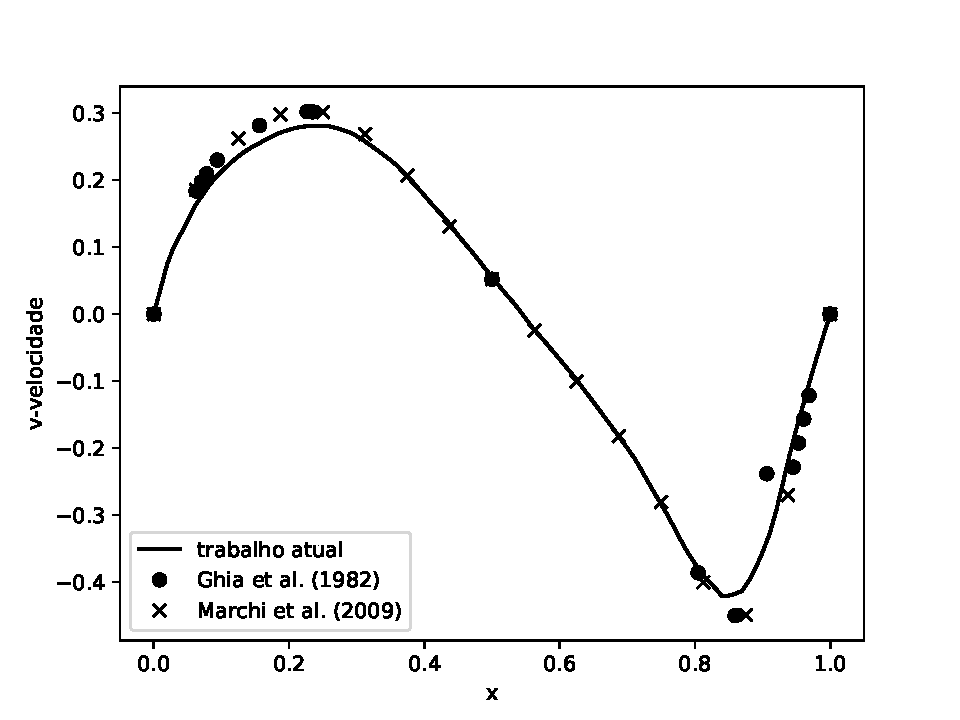
\includegraphics[scale=0.53]{./02_chaps/cap_validation/figure/Re_400_v_profile.pdf}\\
      (c)
     \end{minipage}%
     \begin{minipage}{.5\linewidth}
      \centering
      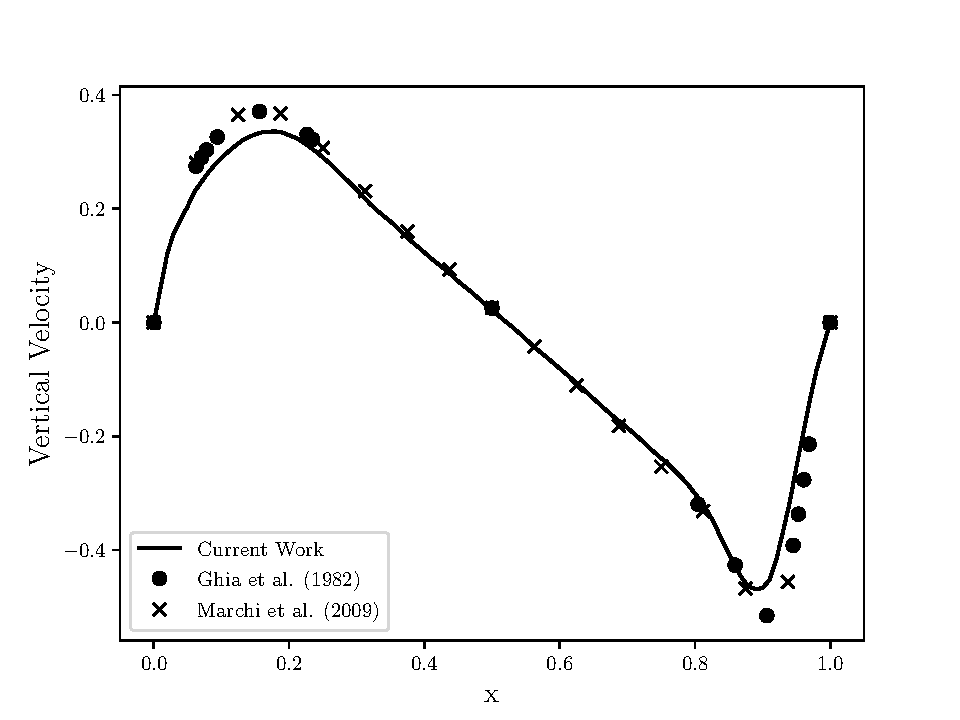
\includegraphics[scale=0.53]{./02_chaps/cap_validation/figure/Re_1000_v_profile.pdf}\\
      (d)
     \end{minipage}
     \medskip
     \caption{Perfil de $v$ na linha central da cavidade ($y=0.5$) com diferentes Reynolds:
     (a) 10
     (b) 100
     (c) 400
     (d) 1000.}
     \label{velocity vy cavity}
\end{figure}

\begin{figure}[H]
     \centering
     \begin{minipage}{.45\linewidth}
      \centering
      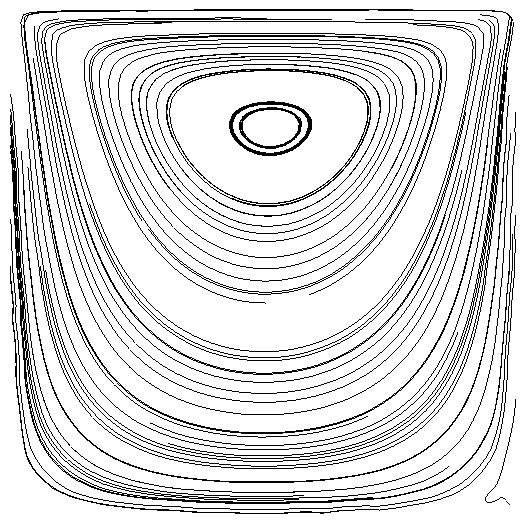
\includegraphics[scale=0.3]{./02_chaps/cap_validation/figure/Re_10_stream_countours.png}\\
      (a)
     \end{minipage}%
     \begin{minipage}{.45\linewidth}
      \centering
      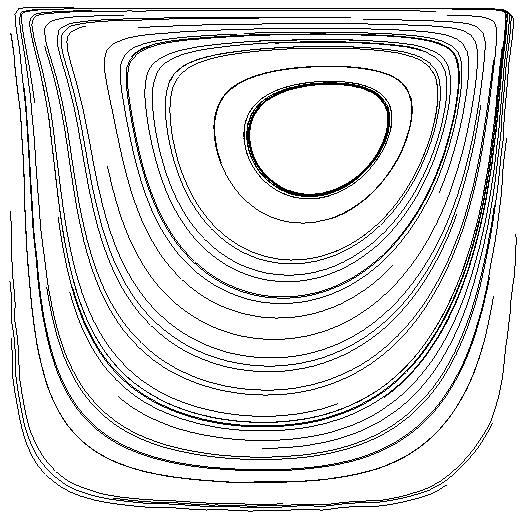
\includegraphics[scale=0.3]{./02_chaps/cap_validation/figure/Re_100_stream_countours.png}\\
      (b)
     \end{minipage}
     \begin{minipage}{.45\linewidth}
      \centering
      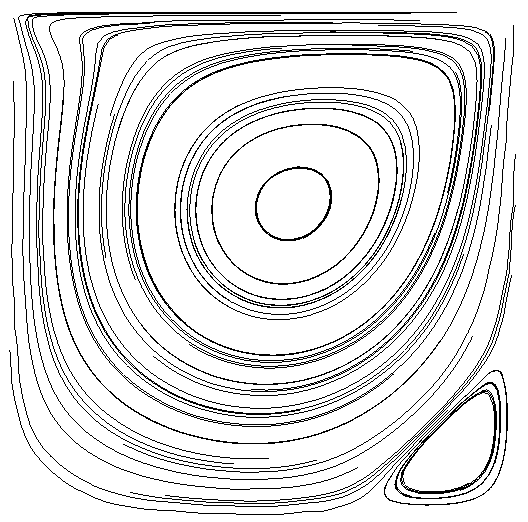
\includegraphics[scale=0.3]{./02_chaps/cap_validation/figure/Re_400_stream_countours.png}\\
      (c)
     \end{minipage}%
     \begin{minipage}{.45\linewidth}
      \centering
      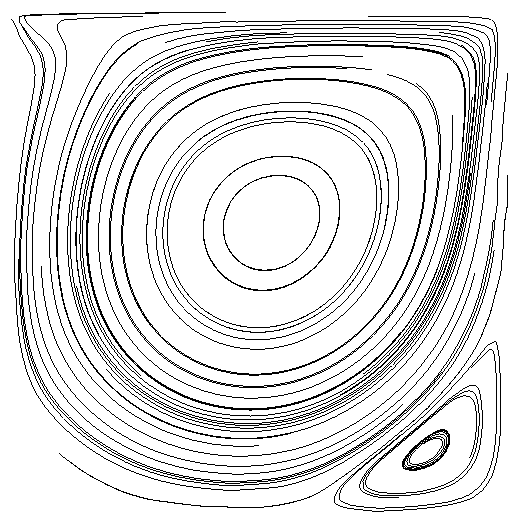
\includegraphics[scale=0.3]{./02_chaps/cap_validation/figure/Re_1000_stream_countours.png}\\
      (d)
     \end{minipage}
     \medskip
     \caption{Os contornos da função de corrente para os Reynolds:
     (a) 10
     (b) 100
     (c) 400
     (d) 1000.}
     \label{countours streamfunction}
\end{figure}


\newpage
